%!TEX root = ../thesis.tex
% ******************************* Thesis Appendix C ****************************
\chapter{User Case Study}
\label{appendix:three:caseStudy}

\ifpdf
    \graphicspath{{Appendix3/Figs/}{Appendix3/Figs/}{Appendix3/Figs/}}
\else
    \graphicspath{{Appendix3/Figs/}{Appendix3/Figs/}}
\fi

The User case study was a 2-week research conducted with 15 students of Paderborn University. 
The study aimed to evaluate the usability of a software application through the use of a survey.
The participants were emailed a user scenario and instructions for joining an online survey. 
The survey lasted 1 hour per participant and was designed to collect feedback on the usability of the software application.
Throughout the 2-week study, the participants were asked to use our software tool and complete a set of tasks while using it. 
They were then asked to provide feedback on their experience using the software application through the online survey.
The survey results were used to assess the software application's overall usability and identify any areas that required improvement. 
The study provided valuable insights into how the software application could be improved to enhance user experience and increase usability. 
Overall, the User case study was a successful project that provided valuable feedback on the usability of the software application.
Out of 15 participants, we present one of the user's prototypes and user scenarios.

\paragraph{Email template:} Here you see the email template (see below) which was sent to every participant before starting the survey.

\paragraph{Survey questionnaire:} Next, see the figure \ref{appendix:fig:sus_sample} to see the first part of the survey questionnaire, figure \ref{appendix:fig:dps_sample} to see the second part of the survey questionnaire, figure \ref{} to see the final part of the survey.
The first part consisted of the SUS questionnaire, whereas, the second part consisted of a scale of 1-5 for rating our \ac{dp}s.
Finally, the last part displays the qualitative questionnaire (see figure \ref{appendix:fig:qualitative_sample}).

\begin{tcolorbox}[title=\texttt{From: Rakshit\\ To: Participant\\ Date: Wed 05/06/2019 15:00\\ Subject: Invitation to participate in a survey}]
Dear Participant,\\
You have been invited to participate in a survey.\\
Please join this BBB room:
\url{https://open-bbb.uni-paderborn.de/b/rak-xtb-6xa-fzz} \\
        
Note: Make sure you are connected to the UPB network or have UPB VPN on.\\

The survey is titled:\\
\textbf{"UI Prototyping tool (Master Thesis)"}\\

\textbf{User Scenario:} Imagine you are John, a UX designer creating a new movie-streaming app for a company. As the UX designer, John is responsible for designing the app's user interface. Unfortunately, John is still determining which UI fits the best for the customers. So, he is looking for solutions where he can prototype the UI and also create split or A/B tests to select the best variant. In the split tests, John wants to create various UI variants and then test the variants with different users and, finally, decide on the best variant from the user feedback. \\

So, John finds an interesting proof of concept tool and logs in as an admin user with the credentials: username - \textit{admin@co.in} \& password - \textit{helloworld}. John finds the tool explanation on the top bar right and checks it. John explores the tool, finds a headstart button that displays (Generate Example UI prototype) on the top bar right and clicks on it to generate an example movie streaming prototype. This headstart option provides a basic layout and a set of UI elements that he can customize. \\
Then, John navigates to the option Data Model in the sidebar on the top left. He finds an already created "movies" model in the data models section. John adds new movies by clicking on the "movies" data model
\dots \\

To participate, please click on the link below.\\
    
Sincerely,\\
Rakshit Bhat\\
(rakshitb@campus.uni-paderborn.de)\\
----------------------------------------------\\
Click here to do the survey:\\
\url{https://umfragen.uni-paderborn.de/index.php/237123?lang=en}
\end{tcolorbox}

\paragraph{SUS Questionnaire:} This is a screenshot (see figure \ref{appendix:fig:sus_sample}) where we had 10 questions for calculating the SUS. 
\begin{figure}[ht]
    \centering
    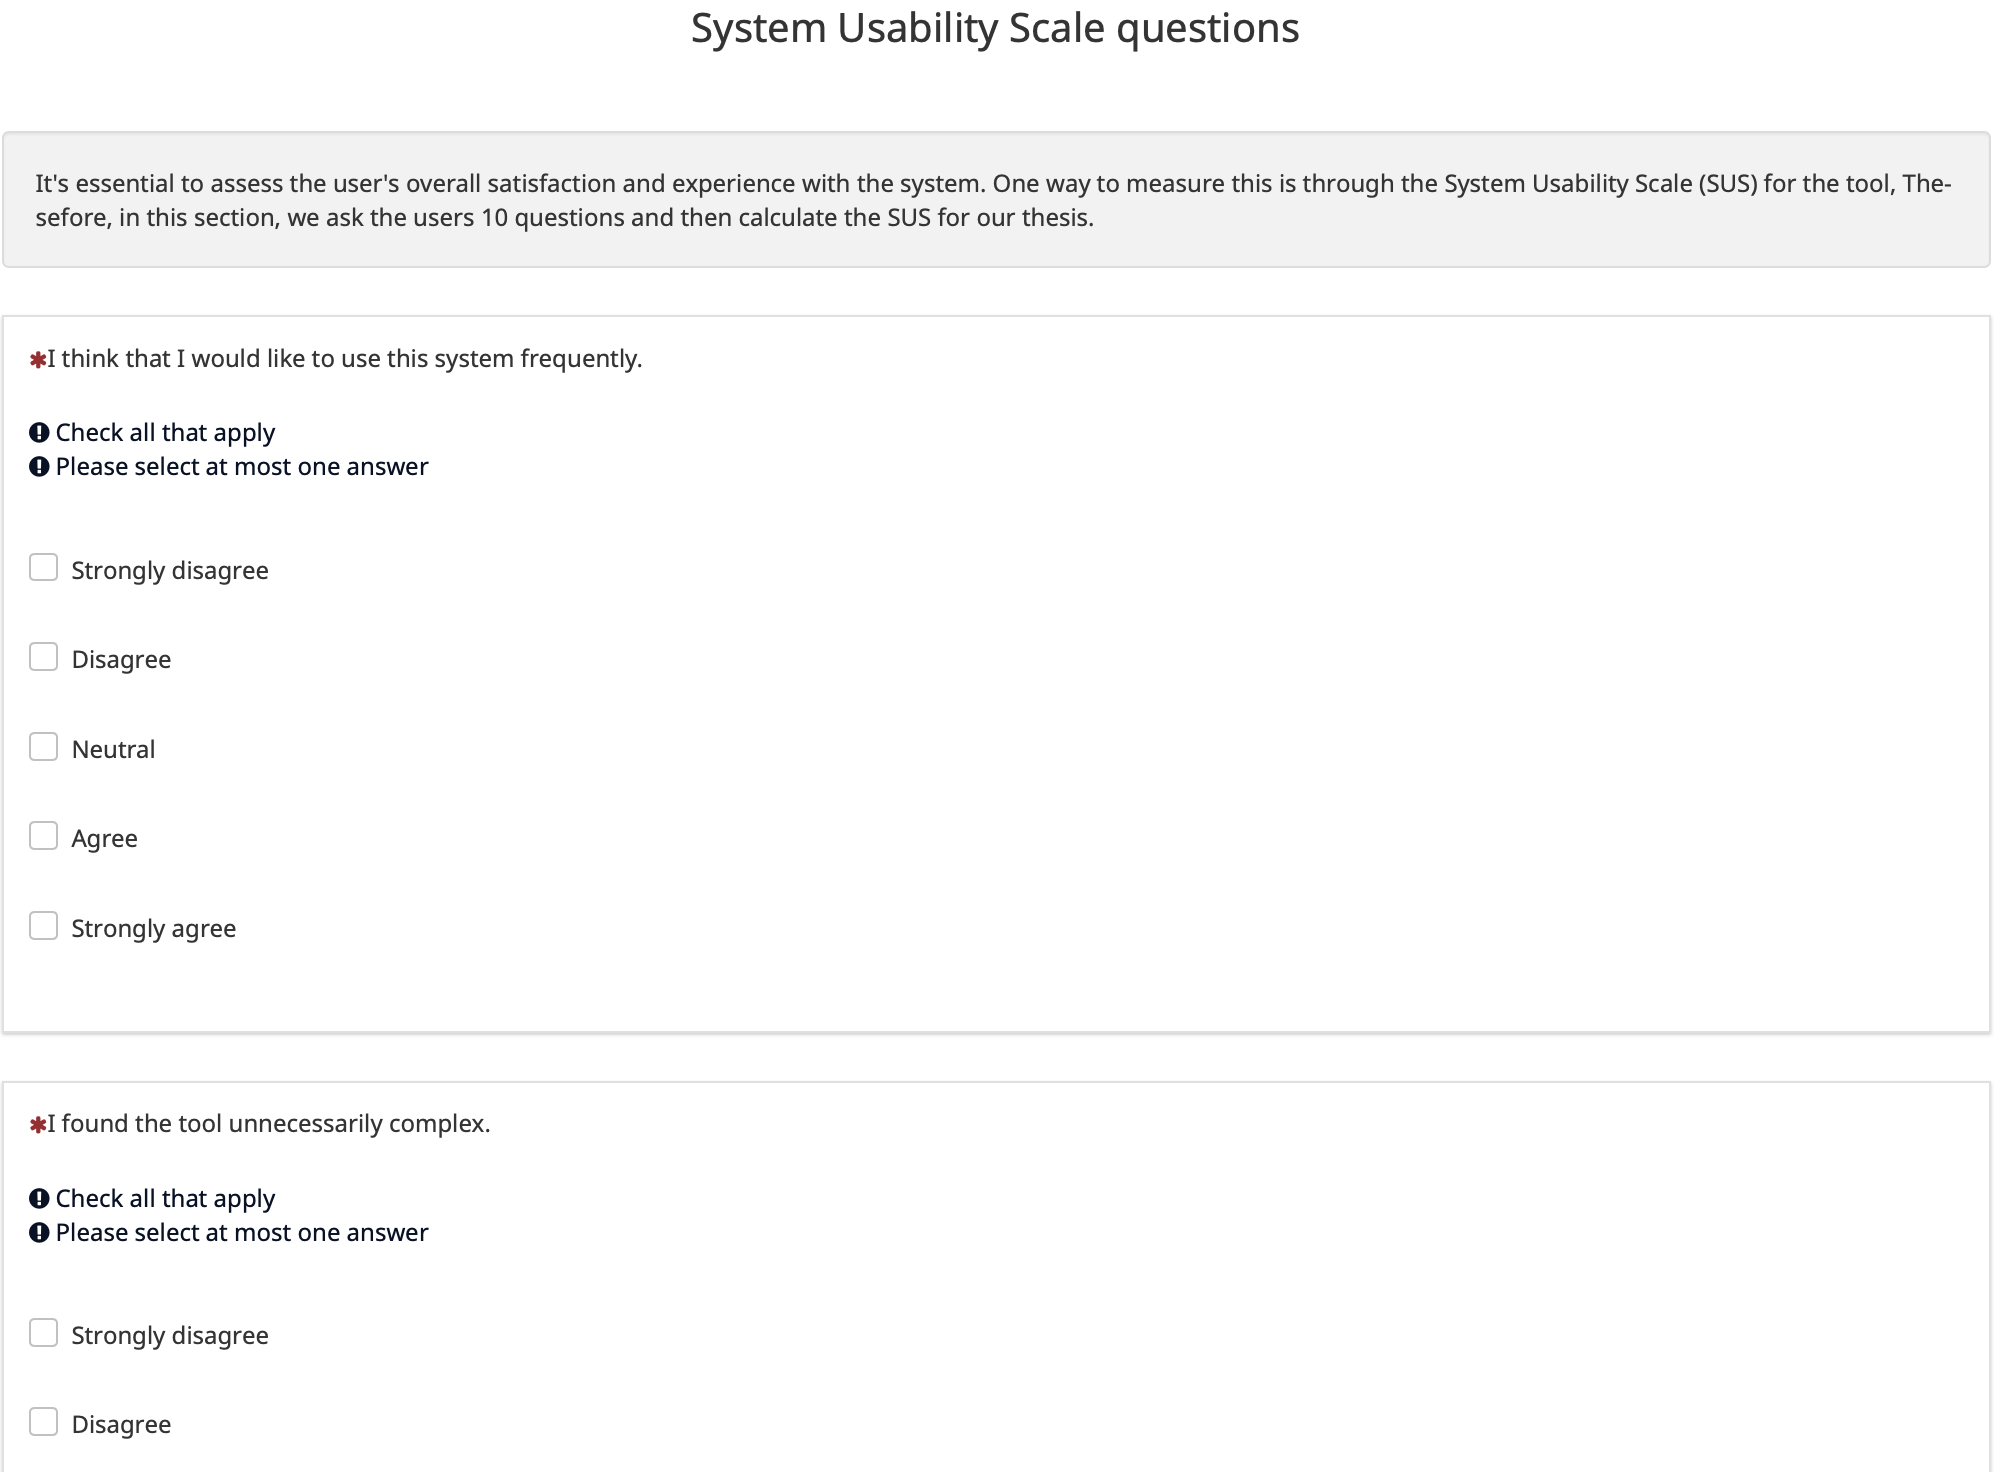
\includegraphics[scale=0.3]{SUS_sample.png}
    \caption[SUS questionnaire]{Survey SUS questionnaire sample}
    \label{appendix:fig:sus_sample}
\end{figure}

\paragraph{DP ratings:} This is a screenshot (see figure \ref{appendix:fig:sus_sample}) where we had a 1-5 scale for rating our \ac{dp}s. 
\begin{figure}[ht]
    \centering
    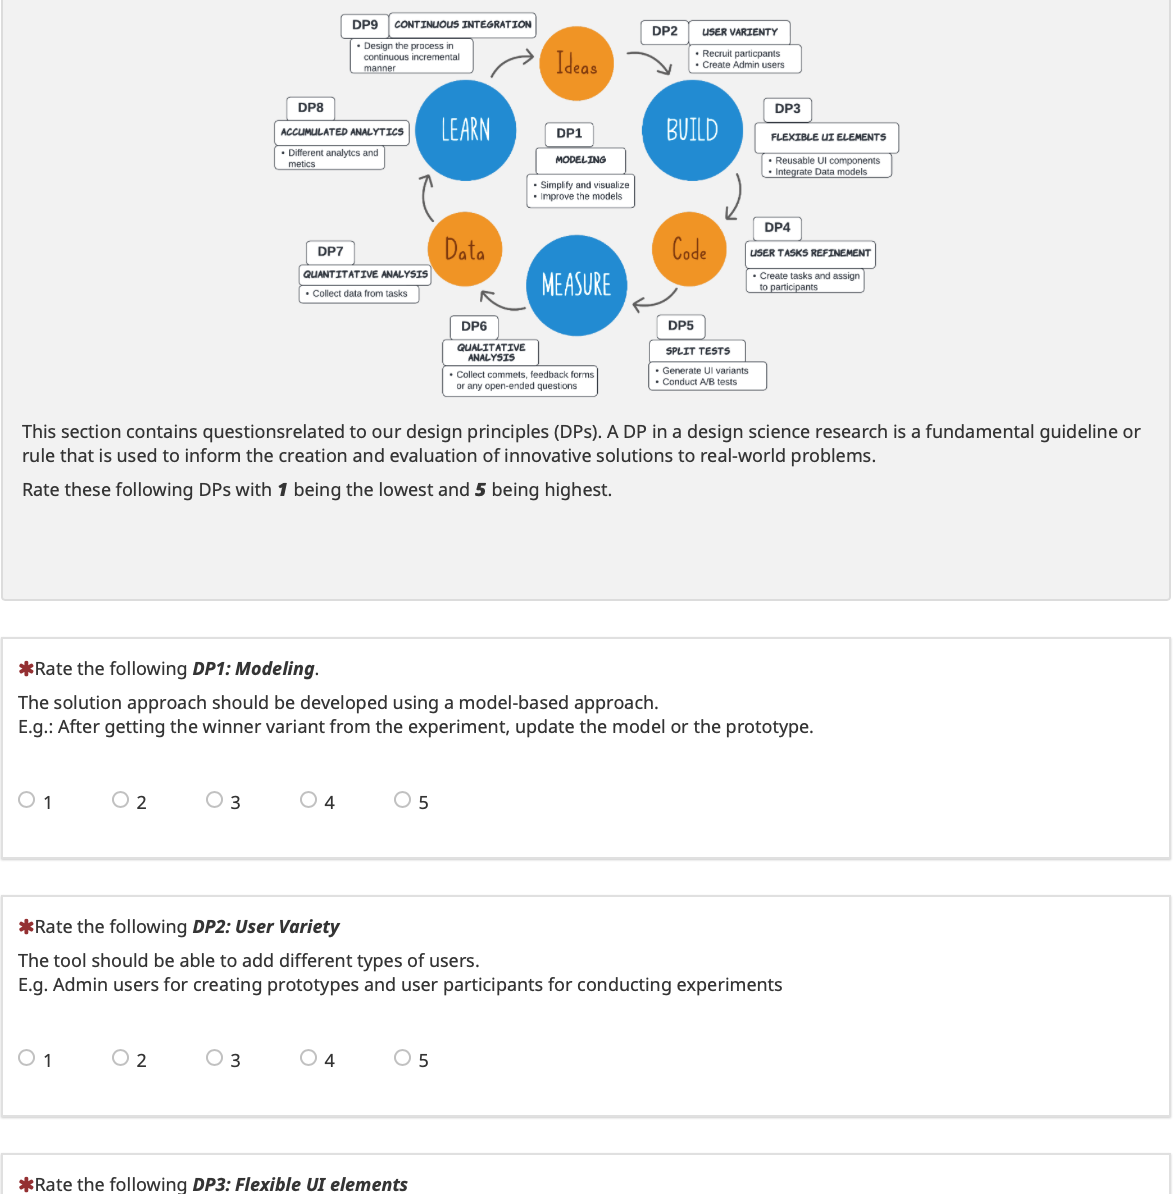
\includegraphics[scale=0.3]{DP_sample.png}
    \caption[DPs questionnaire]{Survey DPs questionnaire sample}
    \label{appendix:fig:dps_sample}
\end{figure}

\paragraph{Open-ended questions:} This is a screenshot (see figure \ref{appendix:fig:sus_sample}) where we had three open-ended questions for rating our tool and our solution approach. 
\begin{figure}[ht]
    \centering
    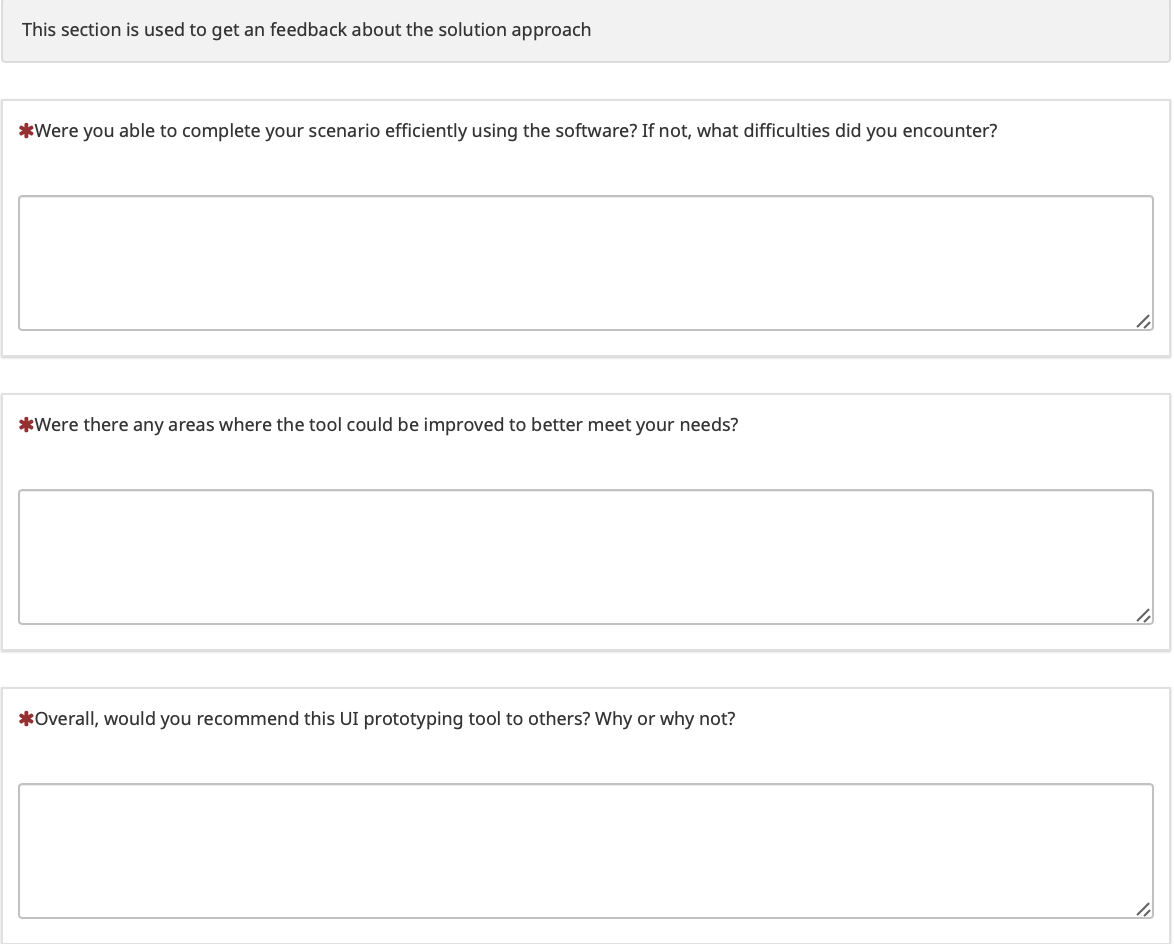
\includegraphics[scale=0.3]{Qualitative_sample.png}
    \caption[Open-ended questionnaire]{Survey Open-ended questionnaire sample}
    \label{appendix:fig:qualitative_sample}
\end{figure}

\paragraph{Example participant prototype:} These are the three screenshots of one of the participant's prototypes that were created. See figure \ref{appendix:fig:masterview}, figure \ref{appendix:fig:gridview}, and figure \ref{appendix:fig:listview}.
\begin{figure}[ht]
    \centering
    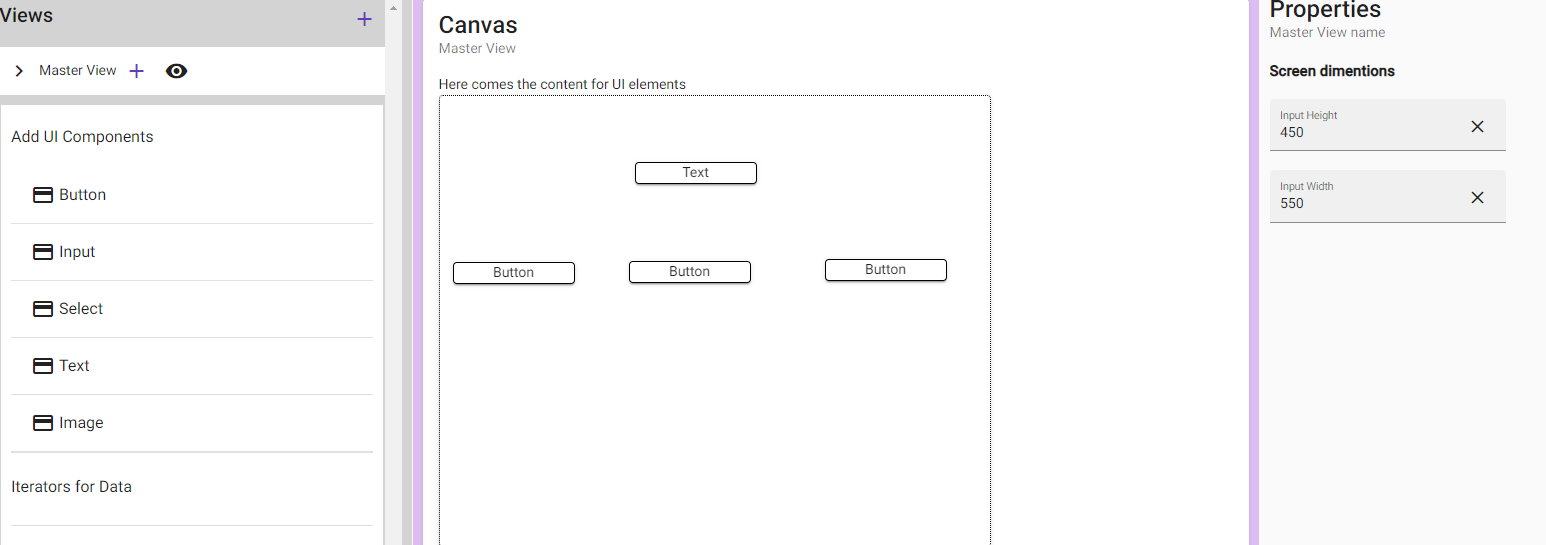
\includegraphics[scale=0.35]{MasterView.png}
    \caption[Example prototype]{Participant Master View}
    \label{appendix:fig:masterview}
\end{figure}

\begin{figure}[ht]
    \centering
    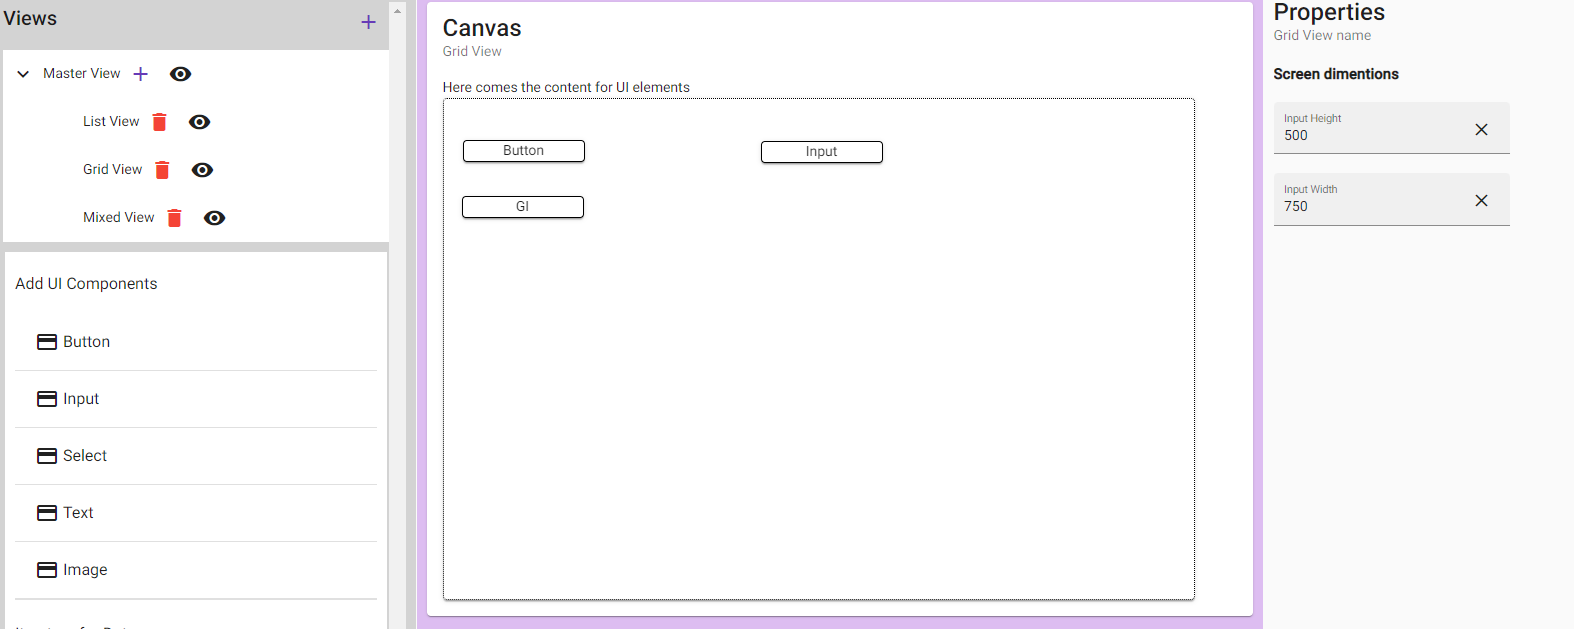
\includegraphics[scale=0.3]{GridView.png}
    \caption[Example prototype]{Participant Grid View}
    \label{appendix:fig:gridview}
\end{figure}

\begin{figure}[ht]
    \centering
    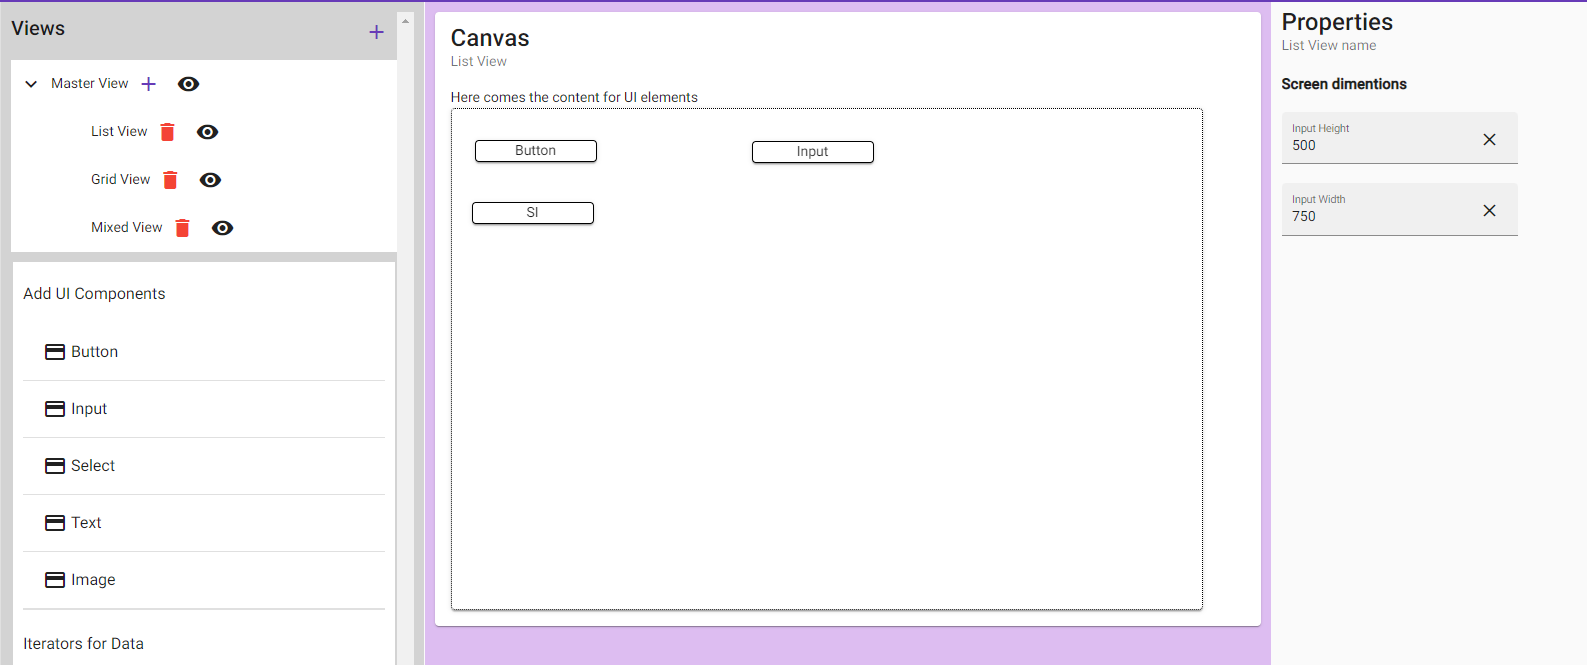
\includegraphics[scale=0.35]{ListView.png}
    \caption[Example prototype]{Participant List View}
    \label{appendix:fig:listview}
\end{figure}

\paragraph{SUS responses:}
These are the SUS responses of all our participants exported from the Survey in a CSV format (see figure \ref{appendix:fig:sus_responses}).
\begin{figure}[ht]
    \centering
    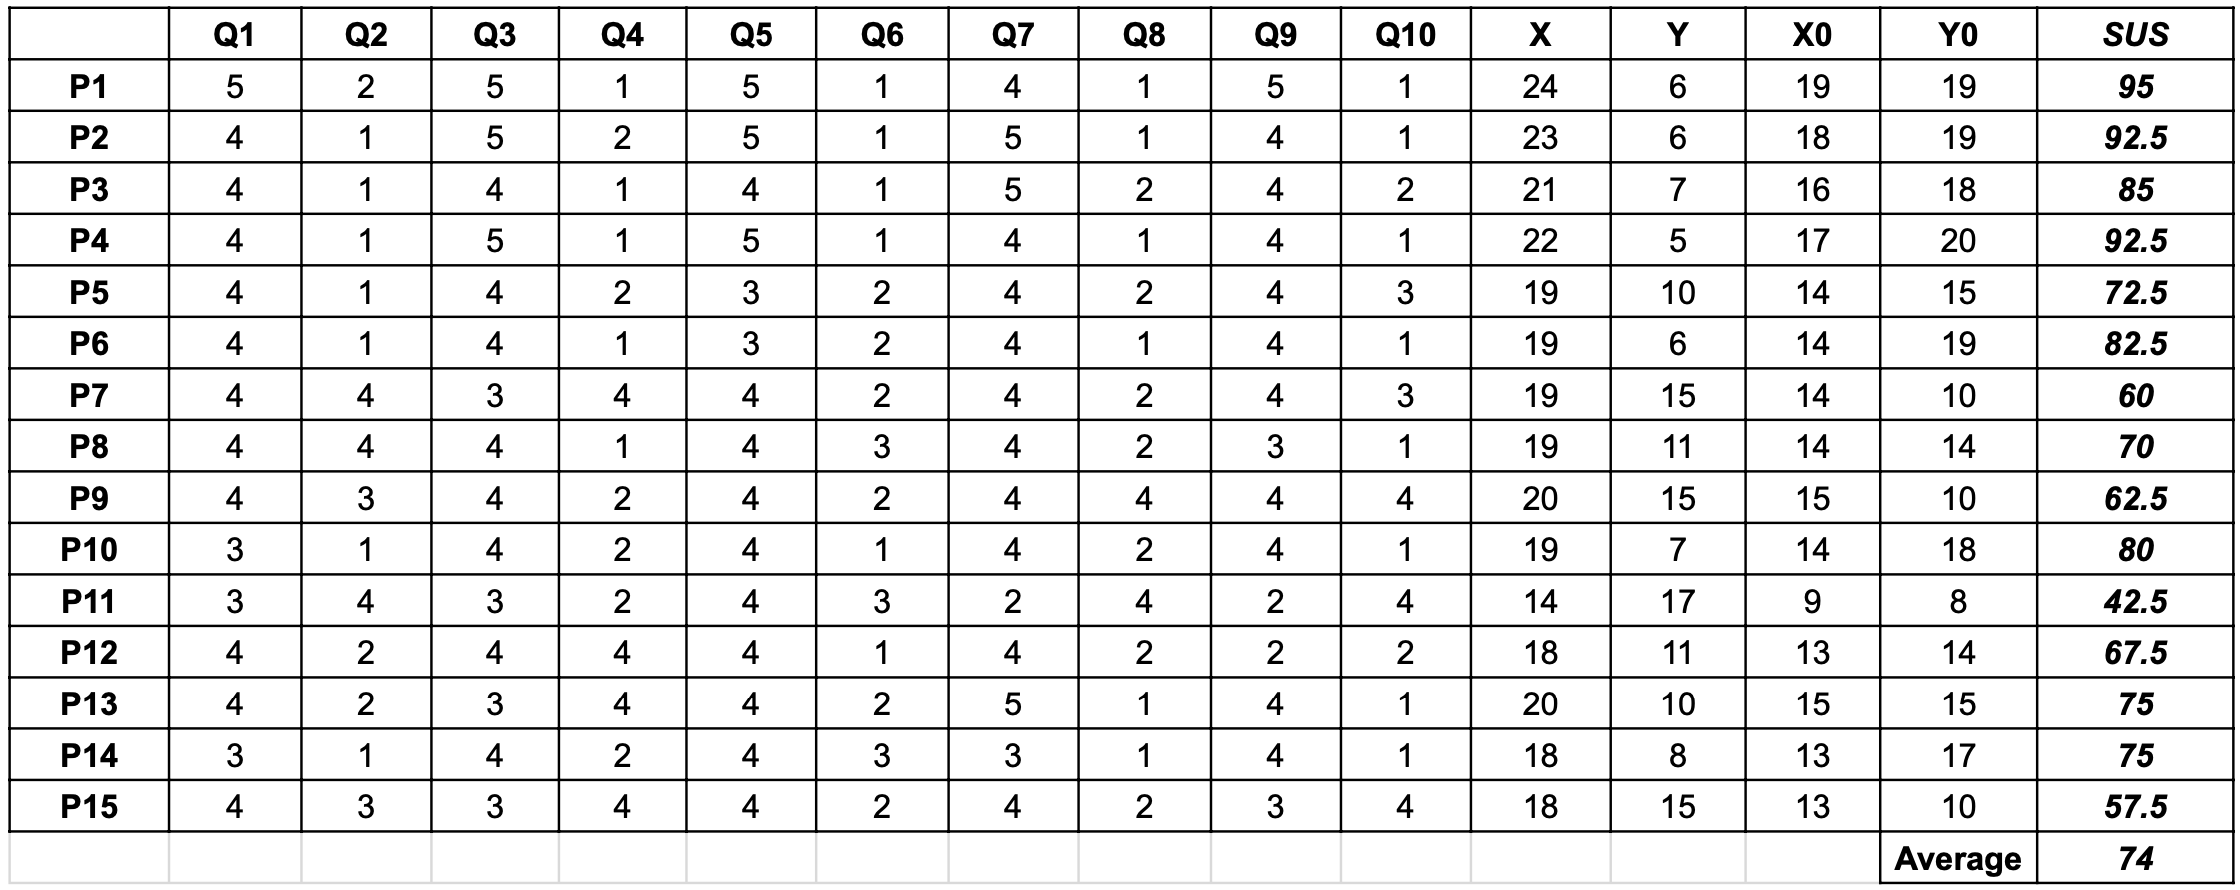
\includegraphics[scale=0.35]{SUS_users.png}
    \caption[SUS responses]{Participant responses SUS}
    \label{appendix:fig:sus_responses}
\end{figure}
\paragraph{DPs responses:}
These are the DPs responses of all our participants exported from the Survey in a CSV format (see figure \ref{appendix:fig:dps_responses}).
\begin{figure}[ht]
    \centering
    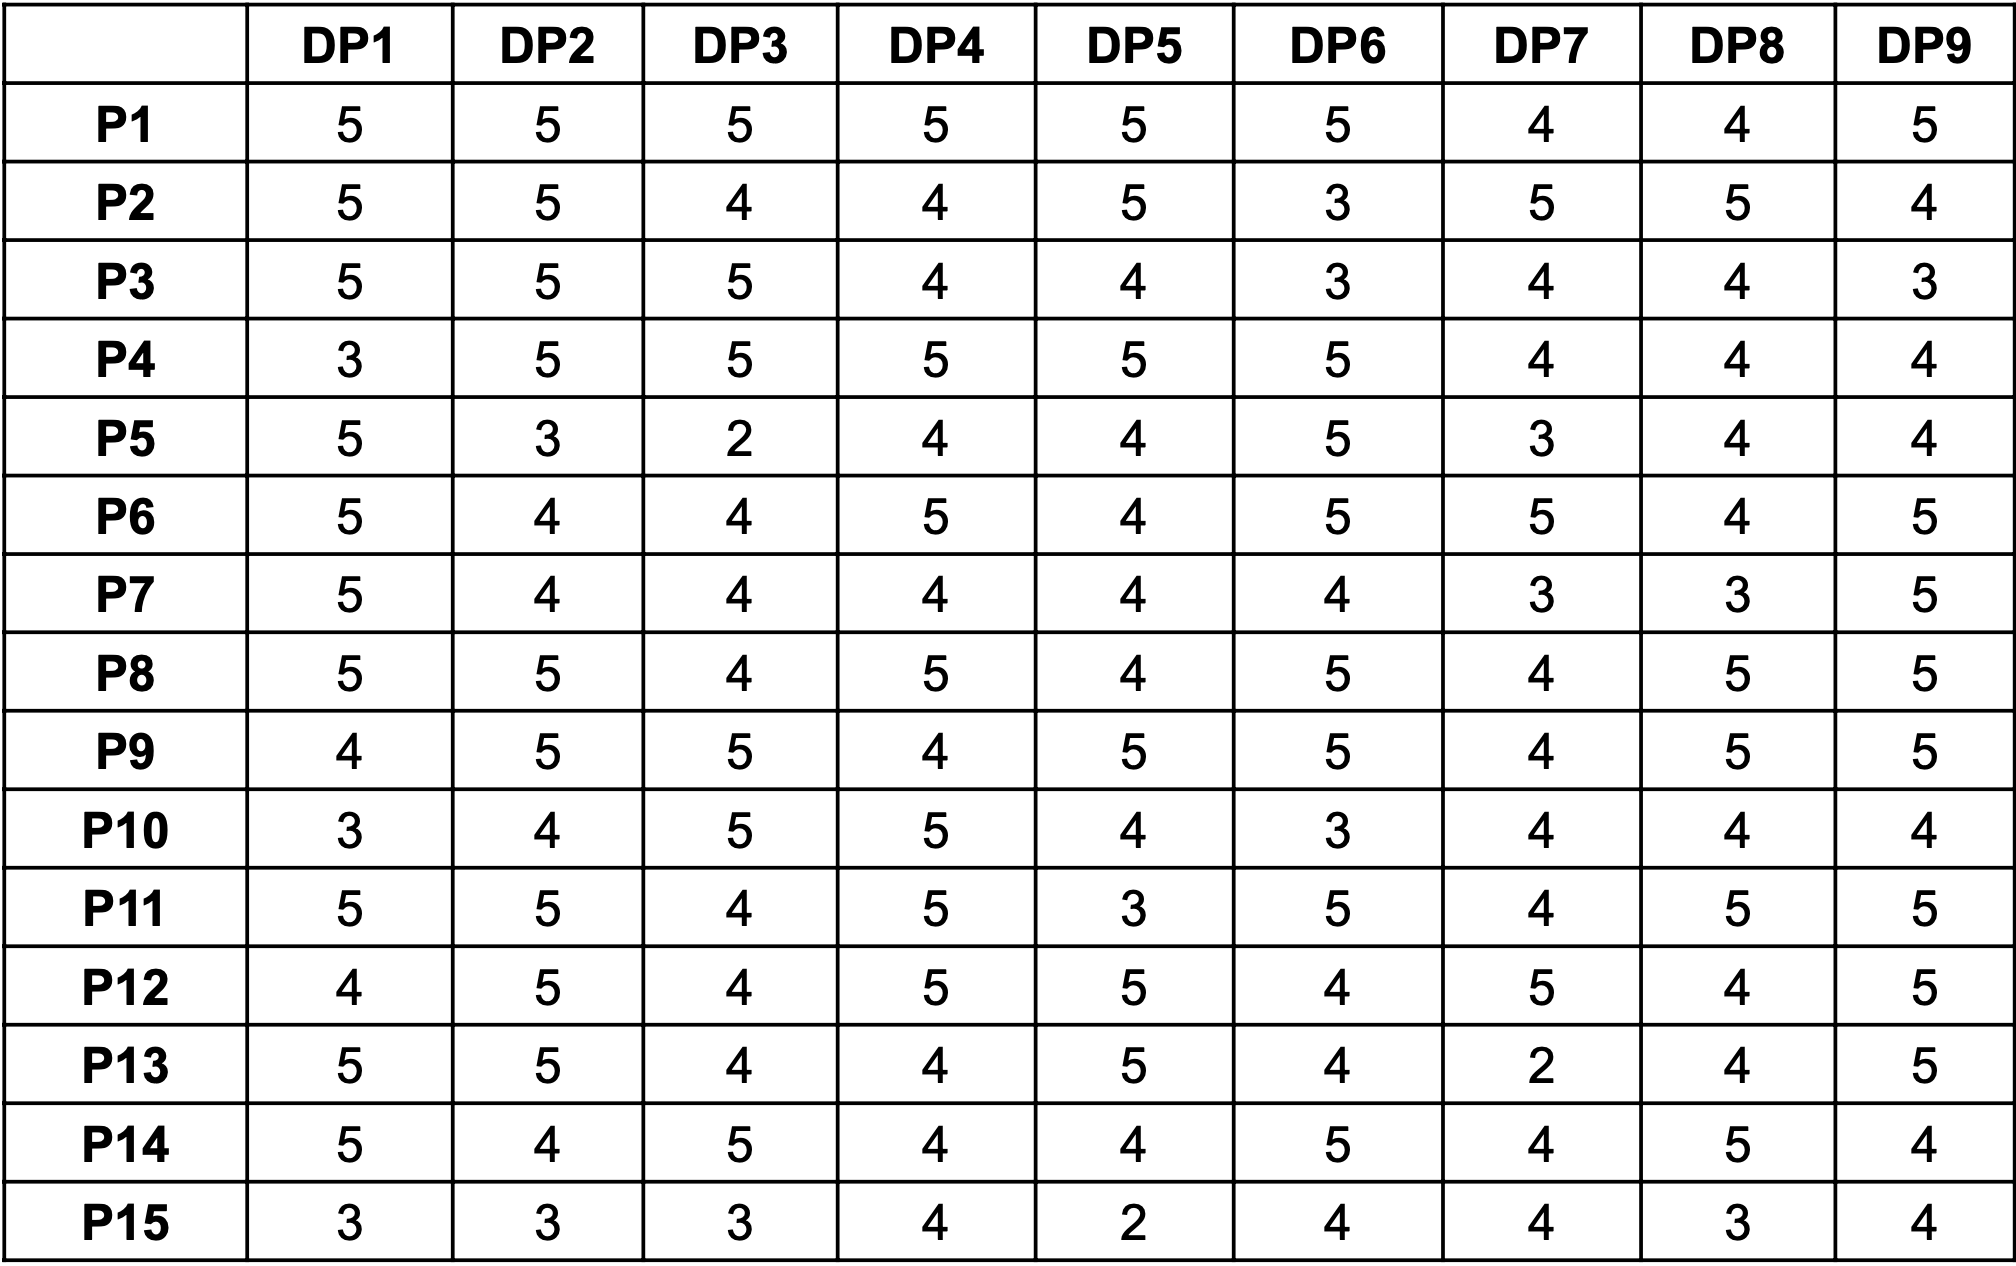
\includegraphics[scale=0.35]{DPs_users.png}
    \caption[DPs responses]{Participant responses DPs}
    \label{appendix:fig:dps_responses}
\end{figure}